\chapter{Theoretical background}
\label{ch:theoreticalbackground}

\section{What is a system?}
\label{sec:tbsystem}

\begin{remark}
	Place standard definitions at this spot of the thesis.
\end{remark}

\subsection{Open vs Closed vs Adaptive systems}
\label{sub:tbopenclosedadaptivesystems}
Complex adaptive system (CAS)\\

Quote from AMS011: \parencite{Turner2019}\\
''The whole is different from the sum of its parts and their interactions'' [61] (p.77) Though emergence, the whole cannot be reduced to the original parts, the whole is considered a new entity or unit. The whole is ''qualitatively different from their parts ... The cannot be meaningfully compared-they are different'' [61] (system holism)\\
CAS is going against the second law of thermodynamics.\\

\subsection{Linear and non-linear systems}
\label{sub:linearnonlinear}

\subsection{Systems of Systems}
\label{sub:systemsofsystems}

\textcite{Maier1996} states that a \acrfull{sos} should be distinguished from large but monolithic systems by the independence of their components, their evolutionary nature, emergent behaviors, and a geographic extent that limits the interaction of their components to information exchange. \textcite{Maier1996} states five principal characteristics, \textcite{Dersin2014} refers to these characteristics as the ''Maier’s criteria'', are useful in distinguishing very large and complex but monolithic systems from true \acrshort{sos}. These five characteristics are:

\begin{itemize}
	\item{\textbf{Operational independence of the elements:} if the \acrshort{sos} is disassembled into its component systems the component systems must be able to usefully operate independently. The	system-of-systems is composed of systems which are independent and useful in their own right.}
	\item{\textbf{Managerial independence of the elements:} The component systems not only can operate independently, they do operate independently. The component systems are separately acquired and integrated but maintain a continuing operational existence independent of the system-of-systems.}
	\item{\textbf{Evolutionary development:} The \acrshort{sos} does not appear fully formed. Its development and existence is evolutionary with functions and purposes added, removed, and modified with experience.}
	\item{\textbf{Emergent Behavior.} The system performs functions and carries out purposes that do not reside in any component system. These behaviors are emergent properties of the entire \acrshort{sos} and cannot be localized to any component system. The principal purposes of the \acrshort{sos} are fulfilled by these behaviors.}
	\item{\textbf{Geographic Distribution.} The geographic extent of the component systems is large. Large is a nebulous and relative concept as communication capabilities increase, but at a minimum it means that the components can readily exchange only information and not substantial quantities of mass or energy.}
\end{itemize}

\begin{remark}
	Goal of this subsection is the buildup to that the public sector is a Systems of Systems.
\end{remark}

\begin{figure}[H]
	\centering
	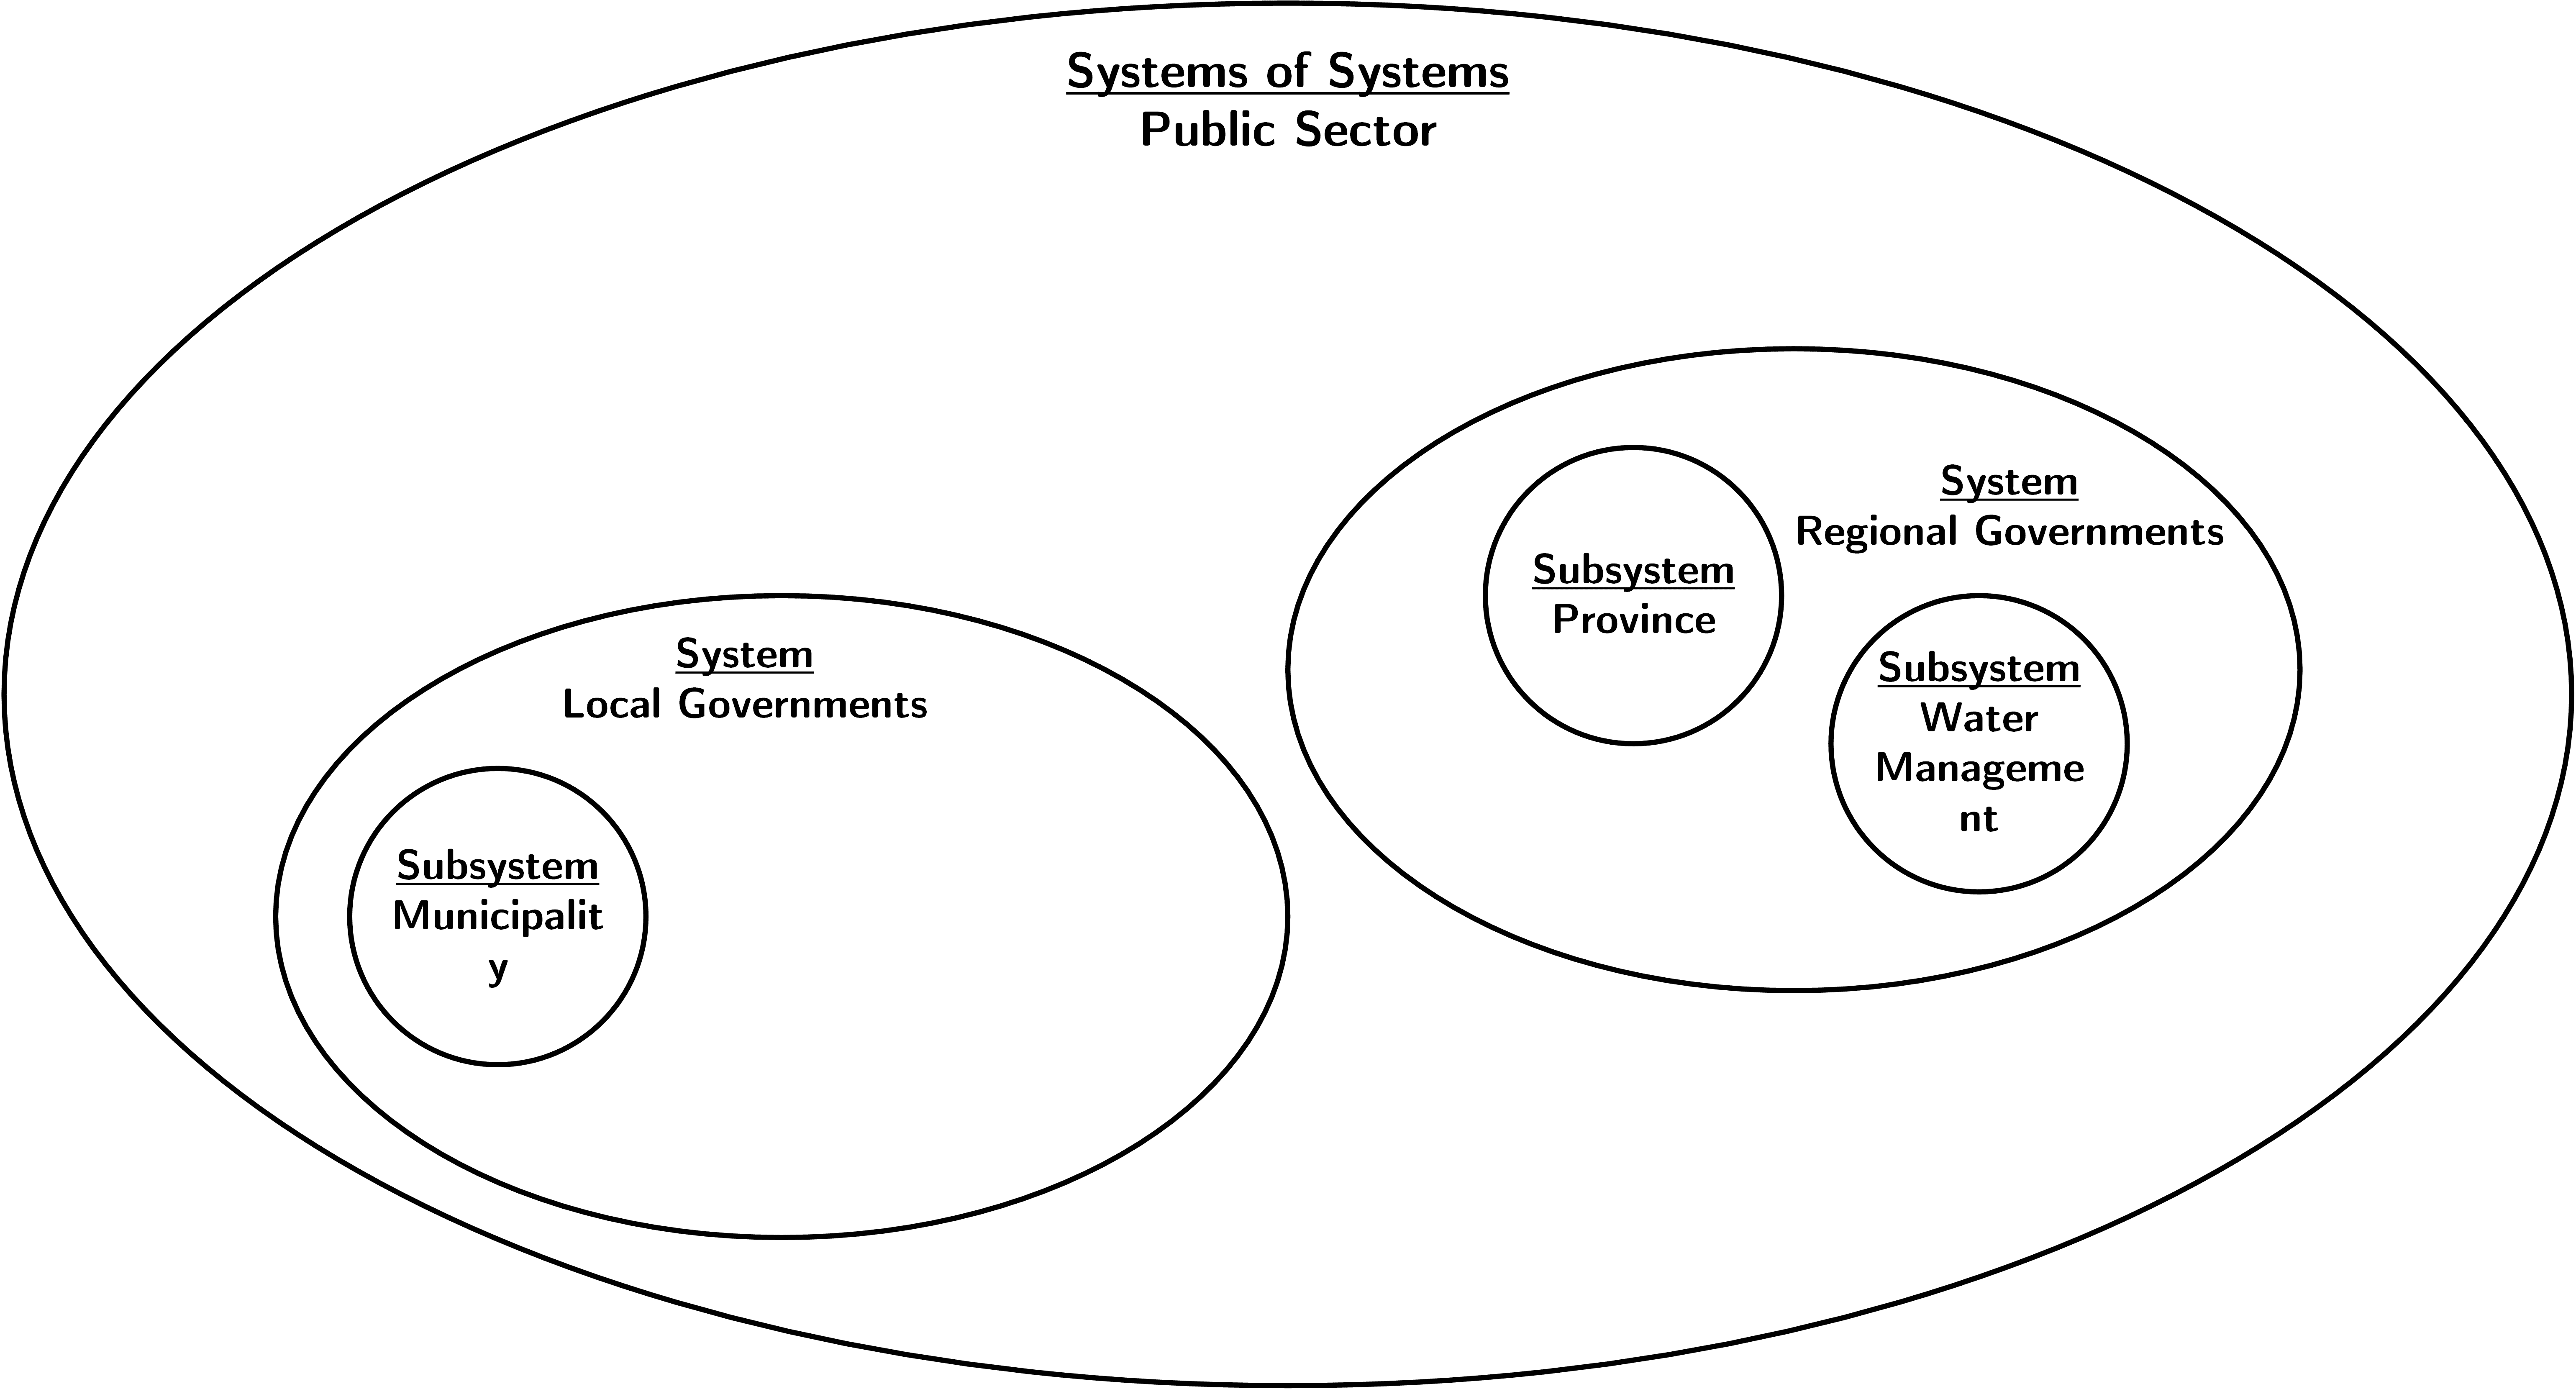
\includegraphics[width=0.7\linewidth]{images/systemsofsystems}
	\caption[Systems of Systems]{Systems of Systems}
	\label{fig:systemsofsystems}
\end{figure}

\subsection{Systems-in-Environment}

\parencite[p. 41]{Lapalme2012}

\subsection{Complexity Theory}
\label{sub:tbcomplexitytheory}
Quote from AMS011:\\
The interactions within organisations are complex and can be explained better through the lens of complexity theory and CAS than by the other theoretical system approaches \parencite[p. 15]{Turner2019}.\\

Consider the concept of the Platonic fold, [7] which tells us that the act of modeling the world
simplifies it to the point where any decisions made based on that model are misinformed due to details omitted for
the sake of hiding complexity. This is also called ‘Hidden Intelligence Syndrome” [ 8]. When humans build complex systems, they tend to fail, often catastrophically, because of Platonic folding. The
solution to the Platonic fold requires accepting complexity as something we can neither predict nor control, along
with accepting the limitations of modeling and risk management. Instead of pursuing correctness in these areas, we
should aim to build systems that are \gls{antifragile} to fluctuations in the \acrshort{vuca} elements (i.e., the system becomes
stronger as the business environment warps and changes with time). \parencite[p. 885]{OReilly2019}

\begin{remark}
	Must elaborate more on this.
\end{remark}

\subsection{Viable Systems Model}
\label{sub:tbvsm}
\acrfull{vsm}


\subsection{Organisation as a System}
\label{sub:tborganisation}

\subsection{To be worked upon}

\begin{itemize}
	\item{Senge (systems theory)}
	\item{Cynefone (systems theory)}
	\item{Seneca's Barbbell (Hydra's Body) (Antifragile)}
	\item{Diversity is a thing of reality and needed.}
\end{itemize}

\section{Antifragile}
\label{sec:tbantifragile}

Antifragile loves both randomness and uncertainty.

\begin{itemize}
	\item{Randomness}
	\item{Variability}
	\item{Hormesis / Mithridatisation (by taleb) / Antidotum Mithridatium}
\end{itemize}

It is important to realize that the degree of \gls{fragility} of a system is often a function of its internal structure. The ability of a system to change under stress is governed by the interconnectedness of its parts, how strongly they are tied to each other, and how much change ripples through the system \parencite[p. 886]{OReilly2019}.\\

''Define antifragility as a property of a system'' \parencite{Jaaron2014}. \textcite{Kastner2017} created a framework for designing an antifragile organisation: Antifragile Organisation Design Framework. The framework consists out of 4 main principles:
\begin{itemize}
	\item{\textbf{Self Organisation.} Decentralisation can be seen as a strategy for organisational survival \parencite{Brafman2007}.}
	\item{\textbf{Ownership.} Result based and 'Skinin the game'.}
	\item{\textbf{Diversity of cells and organisational learning.}}
	\item{\textbf{DNA - Shared purpose, values and culture.}}
\end{itemize}

Decentralised Systems, using self organising capabilities might not only survive disruptions but could even psorsper \parencite{Brafman2007}.The only real difference with Complex Adaptive System and antifragile of \textcite{Taleb2012} is that with antifragile stressors, disruptions, errors, volatility, randomness, chaos and uncertainty are seen as 'desired events' in order to strengten and evolve the system \parencite{Jaaron2014}.\\

To build an antifragile system there are three main concepts to follow \parencite{Russo2017}.
\begin{itemize}
	\item{Since antifragile means to benefit more than to loose (positive asymmetry), the first step is to reduce possible losses.}
	\item{The second step is to avoid disastrous scenarios by hedging correctly risks.}
	\item{The last step is to embed adaptive fault tolerance.}
\end{itemize}

Some authors propose also a fault injection approach, to increase the numbers of errors to enhance the
learning capabilities \parencite{Russo2017}.
\begin{remark}
	This is the method of Antidotum Mithridatium \parencite{Taleb2012}.
\end{remark}

\subsection{What is a stressor?}
\label{sub:stressor}
As \textcite[p. 54]{Taleb2012} points out ''Stress is knowledge (and knowledge is stress).''

\subsection{Volatile, uncertain, complex, and ambiguous}
\label{seb:tbvuca}

\Gls{volatile}, \gls{uncertain}, \gls{complex}, and \gls{ambiguous}.

\subsection{Relation between antifragile, fragile, robust, resilient, and agile}
\label{sub:tbrelatedtoantifragile}

\gls{antifragile} with \gls{fragile}, \gls{robust}, \gls{resilient}, and \gls{agile}.

\subsection{Resilience}
\label{sub:tbresilience}
\textcite[p. 5-7]{MartinBreen2011} distinguishes three types of resilience:
\begin{itemize}
	\item{\textbf{Engineering Resilience.} Bounce back faster after stress, enduring greater stresses, and being disturbed less by a given amount of stress.}
	\item{\textbf{Systems Resilience.} Maintaining system function in the event of a disturbance. Systems resilience has been applied in governance and management, where it is often called robustness.}
	\item{\textbf{Resilience in Complex Adaptive Systems.} The ability to withstand, recover from, and reorganise in repsonse to crisis. The function is maintained by the system structure may not be. The main differentiator is the adaptive capacity or adaptability of the system.}
\end{itemize}

\begin{figure}[h!]
	\centering
	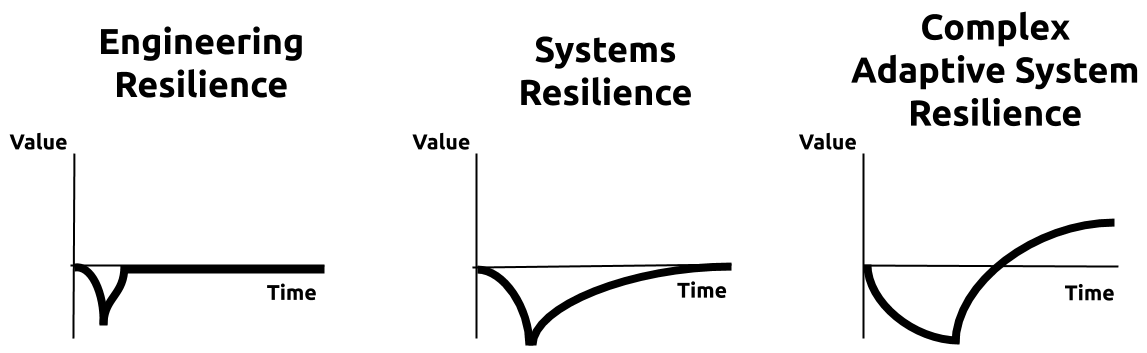
\includegraphics[width=0.7\linewidth]{images/eaal-martin-breen}
	\caption[Three types of resilience]{Three types of resilience \parencite{Botjes2020}}
	\label{fig:eaal-martin-breen}
\end{figure}


\begin{remark}
for systems resilience Kastner loc 327 contains three references that have to be used for reference on robustness.
\end{remark}
Three key sytems properties contribute to its resilience \parencite[p. 9]{MartinBreen2011}:
\begin{itemize}
	\item{Diversity and Redundancy}
	\item{Modular Networks}
	\item{Responsive, regulatory feedbacks.}
\end{itemize}
For resilience one not only needs to answer the questions ''Resilience of what?'' and ''Resilience to what?'', but also ''Resilience for whom?'' \parencite[p. 21]{Lebel2006}. One can apply basic critical systems design principles to spot ways to maintain any system's function in the event of a crisis \parencite[p. 10]{MartinBreen2011}:
\begin{itemize}
	\item{Maintain a diversity of mechanisms to provide identical functions.}
	\item{Make sure networks (social or otherwise) are modular enough so damange or ''infection'' of one portion does not immediately propogate to all others.}
	\item{Maintain or establish feedbacks to, in the simplest case, establish fail0safe mechanisms in case of malfunction.}
\end{itemize}
One can maximize efficiency over all of these variables; however, such optimisation assumes full working knowledge of the system.
\begin{remark}
Enterprise architecture can be used to give this full working knowledge of the system.
\end{remark}

The term resilience (including all three examined concepts) focuses on the avoidance of harmfull stressors and failure; and uncertainty and volatility. Moreover, these are even constructed to reduce vulnerability as much as possible \parencite{MartinBreen2011}.
\begin{remark}
add extra references from Kastner to this cite.
\end{remark}

\subsection{Work of E. A. Botjes}
\textcite{Botjes2020} has conducted literature research for his master project. This literature research was used to define the defintions of \gls{antifragility} and to define attributes relevant to \gls{antifragility}. The outcome of this research is the \acrfull{eaal} model. The outcome of the research of \textcite{Botjes2020} also stated that the attributes of \gls{antifragility} are additional to those of \gls{resiliency}. Therefor \acrshort{eaal} model contains an overview on not only the attributes of \gls{antifragility}.

\begin{figure}[H]
	\centering
	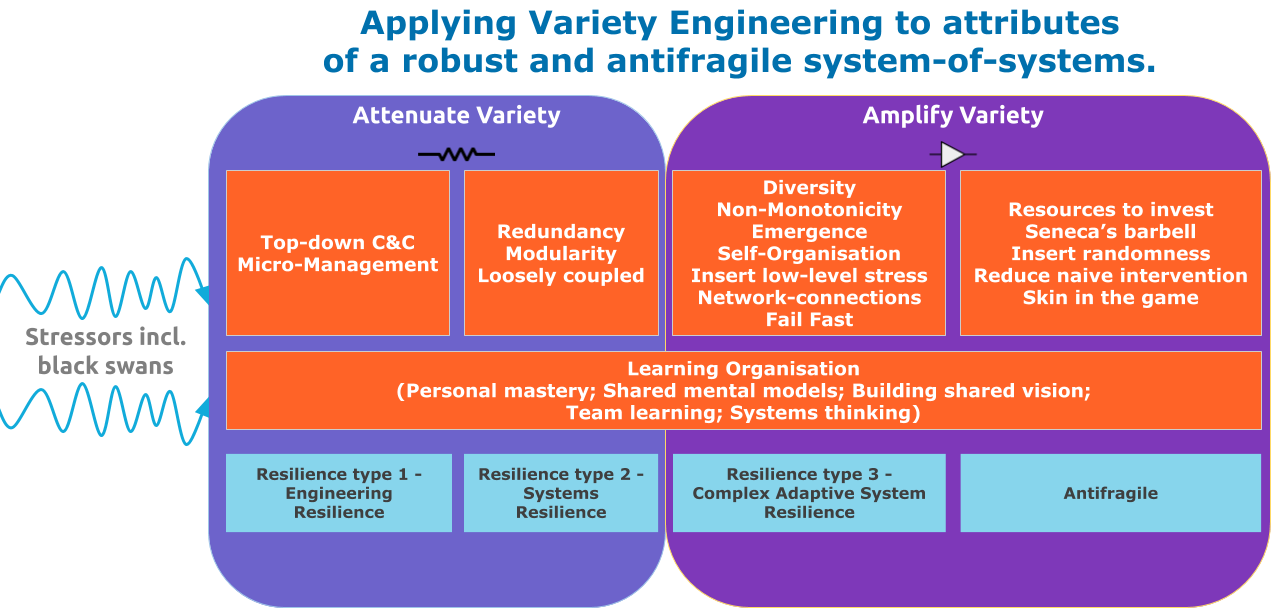
\includegraphics[width=0.7\linewidth]{images/eaal}
	\caption[EAAL]{EAAL \parencite{Botjes2020}}
	\label{fig:eaal}
\end{figure}

The \acrshort{eaal} model of \parencite{Botjes2020} uses Variety Engineering \needsref as his base. The variety engineering consists out of two different varieties. The Attenuate Variety, and the Amplified Variety.

\begin{itemize}
	\item{\textbf{Attenuate Variety.}}
	\item{\textbf{Amplified Variety.}}
\end{itemize}

The more amplified variety a \acrshort{sos} has the more antifragile the \acrshort{sos} is \needsref.

\begin{remark}
Need more information to be eleborated on this. The information should be from the source of Edzo.

Edzo his paper contains references to ashley and beer about these kinds of variety!

\end{remark}

The research of \textcite{Botjes2020} is recent and contains a good overview of needed attributes for a system-of-systems to become more \gls{antifragile}.

\subsection{Antifragile Systems Design}
\label{sub:backgroundasd}

\acrfull{asd} \parencite[p. 886-888]{OReilly2019} requires an organization to move as one toward solving the problem of complexity, which means changing the perspective from “us vs. them” (IT vs. business) to simply “us” (business). Business leaders, business/ enterprise architects, and software architects all need to engage with the process to make it work. This requires a new approach from both architects and business leaders \parencite[p. 886]{OReilly2019}.

\begin{remark}
	Bridge to Business \& IT Alignment of COBIT/EGIT \parencite{DeHaes2020}? Is this a condition before you can start with antifragile? Mention it high level but exclude the application of COBIT in the research.
\end{remark}

Architects need to work with the business to describe the \acrshort{vuca} environment, translate the impacts on the
software decomposition, and even assist in business level mitigations \parencite[p. 886]{OReilly2019}.

\begin{remark}
	Is this only about software systems or also other systems like an organisation? Can it be generalised?
\end{remark}

\textcite[p. 886]{OReilly2019} states that the four important principles for the design of an \gls{antifragile} system, as described by \textcite[p. 35-39]{Hole2016}, are of great importance for \acrshort{asd}.
\begin{enumerate}
	\item{\textbf{Modularity.} Consisting of seperate, linked components.}
	\item{\textbf{Weak Links.} A low level of interconnectedness between components.}
	\item{\textbf{Redundancy.} The presence of more than one component to cope with failure.}
	\item{\textbf{Diversity.} The ability to solve a problem in more than one way with different components.}
\end{enumerate}

The process of \acrshort{asd} constist out of four steps:
\begin{enumerate}
	\item{\textbf{\acrshort{vuca} Analysis.}}
	\item{\textbf{System Decomposition - Flow First Design.}}
	\item{\textbf{Design Testing.}}
	\item{\textbf{Modified \acrfull{fmea}}}
\end{enumerate}
\begin{remark}
	Needs some extra explanation per item
\end{remark}

Going forward, architects should consider the following actions \parencite[p. 889]{OReilly2019}:
\begin{itemize}
	\item{\textbf{Practice VUCA Analysis on the initiative's Business Model.}}
	\item{\textbf{Become an expert in system decomposition.}}
	\item{\textbf{Learn different methods for system decomposition.}}
	\item{\textbf{Learn to use modified \acrshort{fmea} to improve system designs.}}
\end{itemize}

\subsection{Residuality Theory}
\label{sub:residualitytheory}

Resilient systems are, by definition, able to survive disruption and eventually regain function. Beyond resilience is the
idea of antifragility – that systems actually learn from their exposure to stress and become stronger because of it \parencite{Taleb2012}\ \parencite[p. 876]{OReilly2020}. Residuality theory reveals a system as actually being made up of a stack of shadows which we cannot see without turning various lights on and off. We do this through a stressor analysis \parencite[p. 877]{OReilly2020}.

\begin{remark}
	The stack of shadows is related to ''the darkness principle'' \parencite[p. 78]{Richardson2004} from complexity science. This can be replaced with the original source!
\end{remark}

\begin{remark}
	Barry will be contacted for some elaboration on the subject of the residuality theory.\\
	\href{mailto:barry@blacktulip.se}{barry@blacktulip.se}\\
	Twitter: \href{https://twitter.com/technologytulip}{https://twitter.com/technologytulip}
\end{remark}

\section{Enterprise Architecture}
\label{sec:tbea}

\begin{remark}
For example, Ylinen and Pekkola (2018, 2020) recognized two distinct groups of EA experts: a modeling-focused group forming a comprehensive view of an organization and a development-focused group using EA for organizational development. \parencite[p. 16]{Nurmi2021}

Kotusev et al. (2015) reviewed the relevant literature and found three approaches to EA management (EAM): traditional, Massachusetts Institute of Technology (MIT), and dynamic. As discussed by Kotusev et al. (2015), the traditional approach to EAM consists of four phases: documenting the current state, developing the future state, and developing and implementing a transition plan. The MIT approach “advocates the development of a core diagram reflecting a long-term enterprise-level architectural vision.” Finally, the supporting core of the dynamic approach is “just enough, just in time,” meaning no EA is designed until there is a need for it. (Kotusev et al., 2015, p. 4072.)
\end{remark}

There are various understandings of \acrlong{ea} and there is no agreement on them. The various definitions are not always complementary but sometimes in opposite \parencite{Lapalme2012,SaintLouis2019,Hoogervorst2009}.

\textcite{White2018} states that the organisations business requirements guide enterprise architecture — it helps layout how information, business and technology flow together. While \textcite{Gartner} states that Enterprise Architecture is a discipline for proactively and holistically leading enterprise responses to disruptive forces by identifying and analysing the execution of change toward desired business vision and outcomes. EA delivers value by presenting business and IT leaders with signature-ready recommendations for adjusting policies and projects to achieve targeted business outcomes that capitalise on relevant business disruptions. \textcite[p. 9]{Ross2014} defines \acrshort{ea} as the organizing logic for business processes and IT infrastructure, reflecting the integration and standardization requirements of the company’s operating model. The enterprise architecture provides a long-term view of a company’s processes, systems, and technologies so that individual projects can build capabilities—not just fulfill immediate needs. \textcite[p. 24]{Greefhorst2011} defines \acrshort{ea} as those properties of an enterprise that are necessary and sufficient to meet its essential requirements.

\subsection{Three schools of Enterprise Architecture}
\label{sub:eathreeschools}
There are three schools of Enterprise Architecture \parencite{Lapalme2012}:
\begin{itemize}
	\item{\textbf{Enterprise IT Architecting.} Inputs are business strategy and objectives.}
	\item{\textbf{Enterprise Integrating.} It is grounded in systems thinking. It has a holistic view. The link between strategy and execution. Inputs are business strategy and objectives.}
	\item{\textbf{\acrfull{eea}.} Fostering organisational learning by designing all facets of the enterprise, including the relation to its environment.}
\end{itemize}

 \textcite{Lapalme2012} defined the scope of \acrshort{eea} ''the enterprise in its environment, including not only the enterprise but also its environment and the bidirectional relationship and transactions between the enterprise and its environment'' with the purpose to ''help the organization innovate and adapt by designing the various enterprise facets to maximize organizational learning throughout the enterprise.'' As \textcite{Botjes2020} concluded with his \acrshort{eaal} model the attribute learning organisation is of importance for being \gls{resilient} or \gls{antifragile}. If the learning organisation is one of the conditions to be \gls{antifragile} the practice of \acrshort{ea} should be of the school of \acrshort{eea}. \textcite[p. 42]{Lapalme2012} states that the following authors are in the school of \acrshort{eea}:
 
 \begin{table}[H]
 	\centering
 	\begin{tabular}{p{0.4\textwidth}p{0.4\textwidth}}
 		\toprule
 		Jamshid Gharajedaghi & Tom Graves \\%
 		Jan Hoogervorst	& James Martin \\%
 		Kevin Smith & James Lapalme\\%
 		Donald de Guerre &  \\%
 		\bottomrule
 	\end{tabular}
 	\caption{\acrshort{eea} authors}
 	\label{tab:eeaauthors}
 \end{table}

The properties of an \acrshort{eea} are:

\begin{longtable}{p{.2\textwidth}p{.8\textwidth}}
	\toprule
	& \textbf{\acrlong{eea}} \\ \midrule%
%	\multicolumn{2}{c}{\textbf{\acrlong{eea}}} \\ \midrule%
	\endhead%
	\hline
	\caption{\acrlong{eea}}
	\label{tab:eaeea}	
	\endfoot%
	Motto    		& Enterprise architecture is the means for organizational innovation and sustainability \\
	Objectives and 	& Innovate and adapt    \\
	concerns		& Support organizational coherence \\
					& Encourage system-in-environment coevolution \\
	Principles and  & Apply a holist (systemic) stance \\
	assumptions		& System-in-environment coevolution  \\
					& Environment can be changed \\
					& Jointly design all organisational dimensions \\
	Skills 			& Foster dialogue \\
					& Apply system and system-in-environment thinking \\
	Challenges		& Foster sensemaking \\
					& Encourage systems thinking and systems-in-environment paradigm shifts \\
					& Collaborate across the organisation \\
	Insights		& Fosters system-in-environment coevolution and enterprise choherency \\
					& Fosters organisational innovation and sustainability \\
	Limitation		& Requires many organisational preconditions for management and strategy creation \\
	\bottomrule
\end{longtable}

\subsection{Steering mechanisms}
\label{sub:tbeasteering}

\section{Public sector}
\label{sec:tbpsmarket}

\subsection{Differences with the Private Sector Market}
\label{sub:tbdifferenceprivatesector}
